\documentclass[12pt, a4paper]{report}

\usepackage{listings}           \usepackage{graphicx}
\usepackage{geometry}           \usepackage{etoolbox}
\usepackage{parskip}            \usepackage{caption}
\usepackage{subcaption}         \usepackage{hyperref}
\usepackage{lmodern}            \usepackage{minted}
\usepackage{array}              \usepackage{listings}
\usepackage{xcolor}             \usepackage{pdfpages}
\usepackage[utf8]{inputenc}     
\usepackage[T1]{fontenc}
\usemintedstyle{xcode}
\lstset { %
    language = C++,
    backgroundcolor=\color{black!5}, % set background colour
    basicstyle=\footnotesize,% basic font setting
}
\definecolor{LightGray}{gray}{0.9}
\definecolor{Arsenic}{rgb}{0.1, 0.1, 0.1}
%=================================================================
\makeatletter
% \patchcmd{<cmd>}{<search>}{<replace>}{<success>}{<failure>}
% --- Patch \chapter
\patchcmd{\@makechapterhead}{50\p@}{\chapheadtopskip}{}{}% Space from top of page to CHAPTER X
\patchcmd{\@makechapterhead}{20\p@}{\chapheadsep}{}{}% Space between CHAPTER X and CHAPTER TITLE
\patchcmd{\@makechapterhead}{40\p@}{\chapheadbelowskip}{}{}% Space between CHAPTER TITLE and text
% --- Patch \chapter*
\patchcmd{\@makeschapterhead}{50\p@}{\chapheadtopskip}{}{}% Space from top of page to CHAPTER TITLE
\patchcmd{\@makeschapterhead}{40\p@}{\chapheadbelowskip}{}{}% SPace between CHAPTER TITLE and text
\makeatother
% Set new lengths
\newlength{\chapheadtopskip}\setlength{\chapheadtopskip}{0pt}
\newlength{\chapheadsep}\setlength{\chapheadsep}{10pt}
\newlength{\chapheadbelowskip}\setlength{\chapheadbelowskip}{10pt}

\newgeometry{
    top=2cm,
    bottom=2cm,
    outer=1.5cm,
    inner=1.5cm,
}
%=================================================================
\title{CPS2000 - Compiler}
\author{Keith Farrugia}
\date{May 2024}

\begin{document}

\maketitle
\tableofcontents

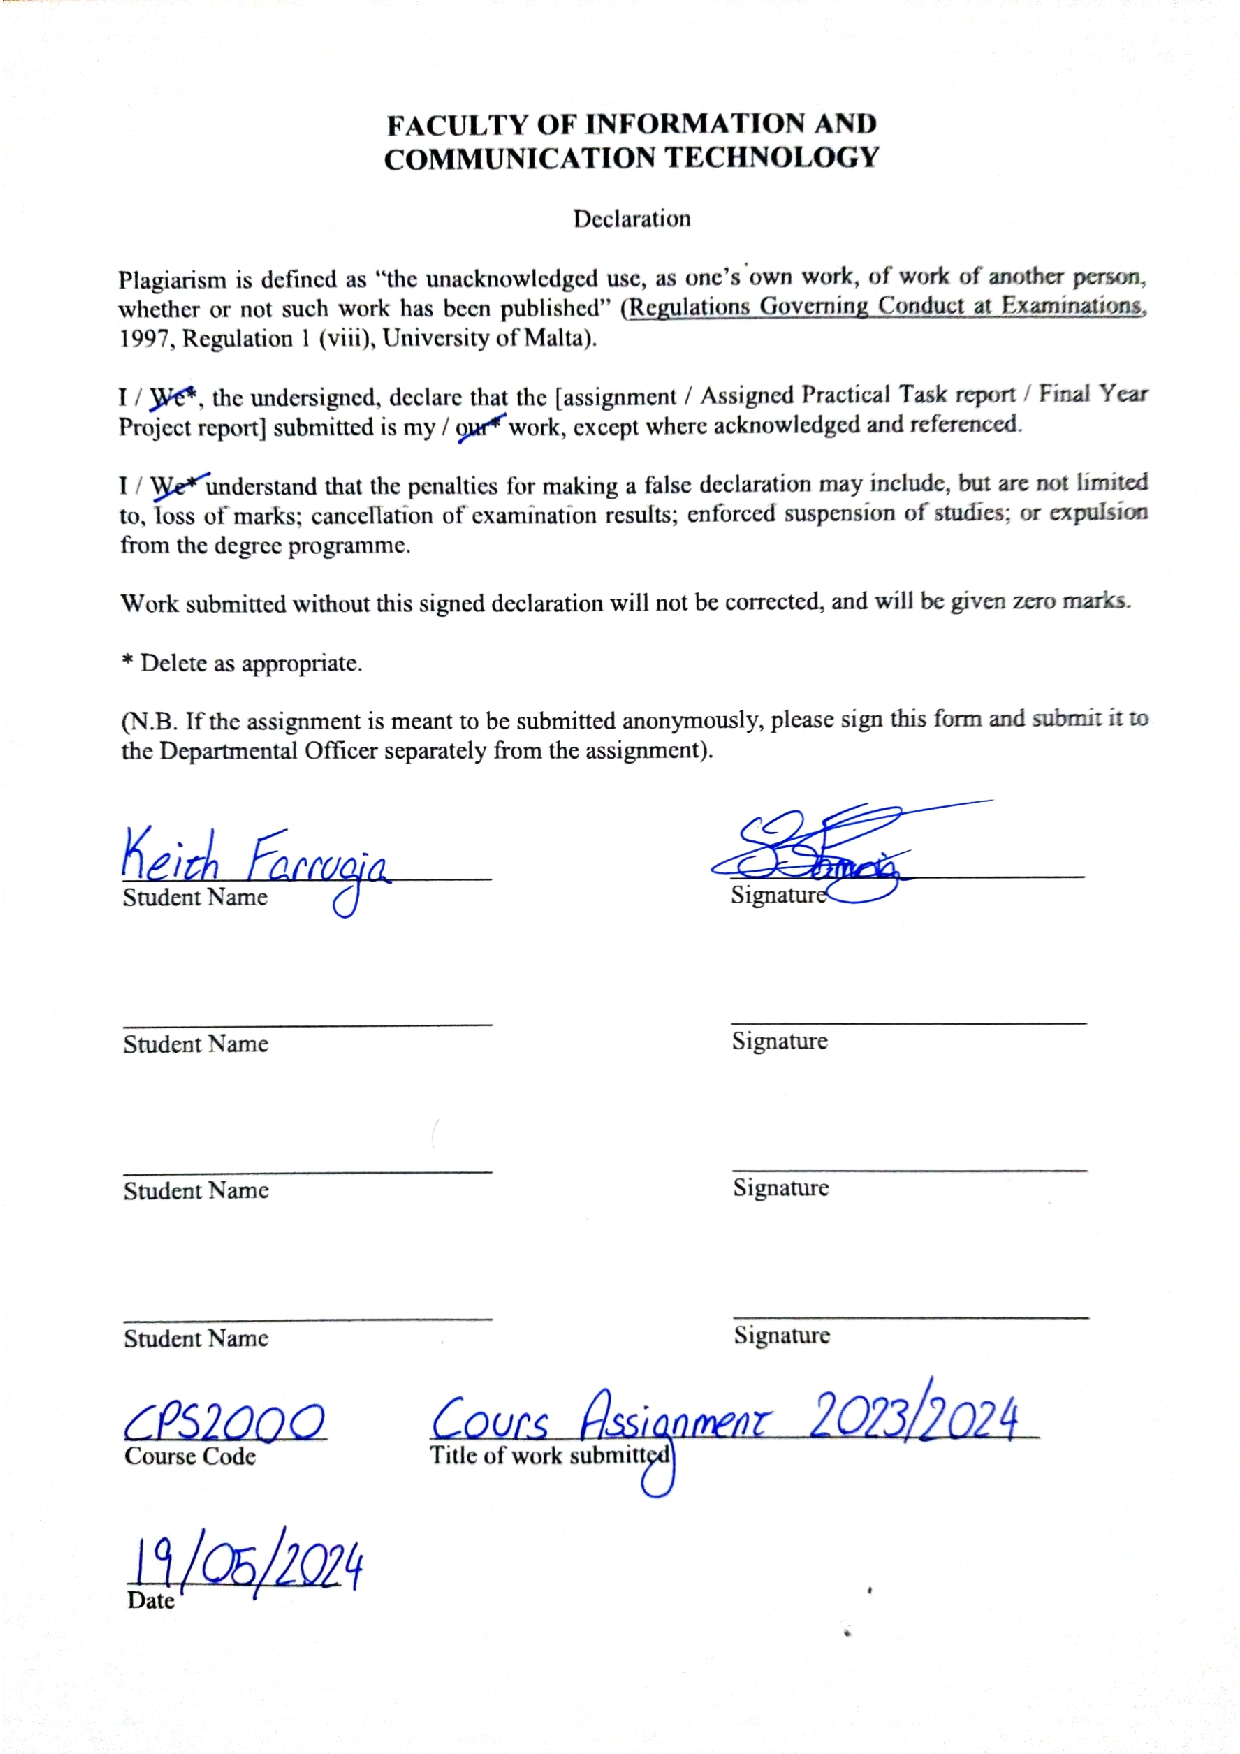
\includepdf[pages={1}]{Plagiarism Form - Keith Farrugia 11104L.pdf}

\chapter{Introduction}
\section{Basic Structure}
The Structure of the code repository is pretty straightforward. Each listed task is contained in its folder excluding task 5 which required changes in the previous task's implementation rather than having its folder. Each task also has its own "Tester" executable. 

This is used to test the current task's implementation and follow a stagard effect where of course the later the "Tester" the more tasks it is using, meaning that although the "Semantic\_Tester.cpp" is mostly there to test semantic cases, it is using both the Lexer and Parser implementations from the previous tasks. The only task that doesn't follow this pattern is Code Generation because the code generation tester would include the use of all functions which is effectively the finished Compiler. 

"Test\_Benches" holds the code to be flexed, parsed, semantically checked, or fully compiled by the respective Tester. In the case of code generation, the compiled code is stored in the "CompiledBuild" folder. 

The "Utility" folder is the folder used commonly by each task, holding information such as the enums, common structures, and functions relating to them or for general use.

\section{Report Structure}
Concerning the report, it is split into sections, one per task. This exception is only for the tasks related to arrays. This is because arrays aren't an extra component which is attached to the rest such as the code generator visitor. Hence arrays will be discussed throughout the other sections as they where more so integrated into them rather then separate.

On another note, the report does not handle the direct explanation of the code. This is because the code itself is too long for an explanation to fit in this report. Hence it will serve more to discuss general concepts and deviations from the original requirements.

% ==================================================================================
%                   Lexer
% ==================================================================================

\chapter{Lexer}

The Lexer works on the premise of a DFSA to read characters and convert them into tokenized strings. The mentioned DFSA can be seen in graph form in the figure below [Figure: \ref{DFSA}].

\section{DFSA} 
One important thing to note is the "ST\_SYNTAX\_ERROR" nodes, these are used in certain edge cases due to how the Lexer was implemented. Take the example "123abc", without the error nodes the lexer would deduce the integer "123" and the identifier "abc", but since there is no space or other symbol this deduction would be semantically incorrect. Hence these States were created to force the lexer to be more thorough when it comes to the semantic structure of the string/program being lexically analysed

\begin{figure}[!htp]
    \centering
    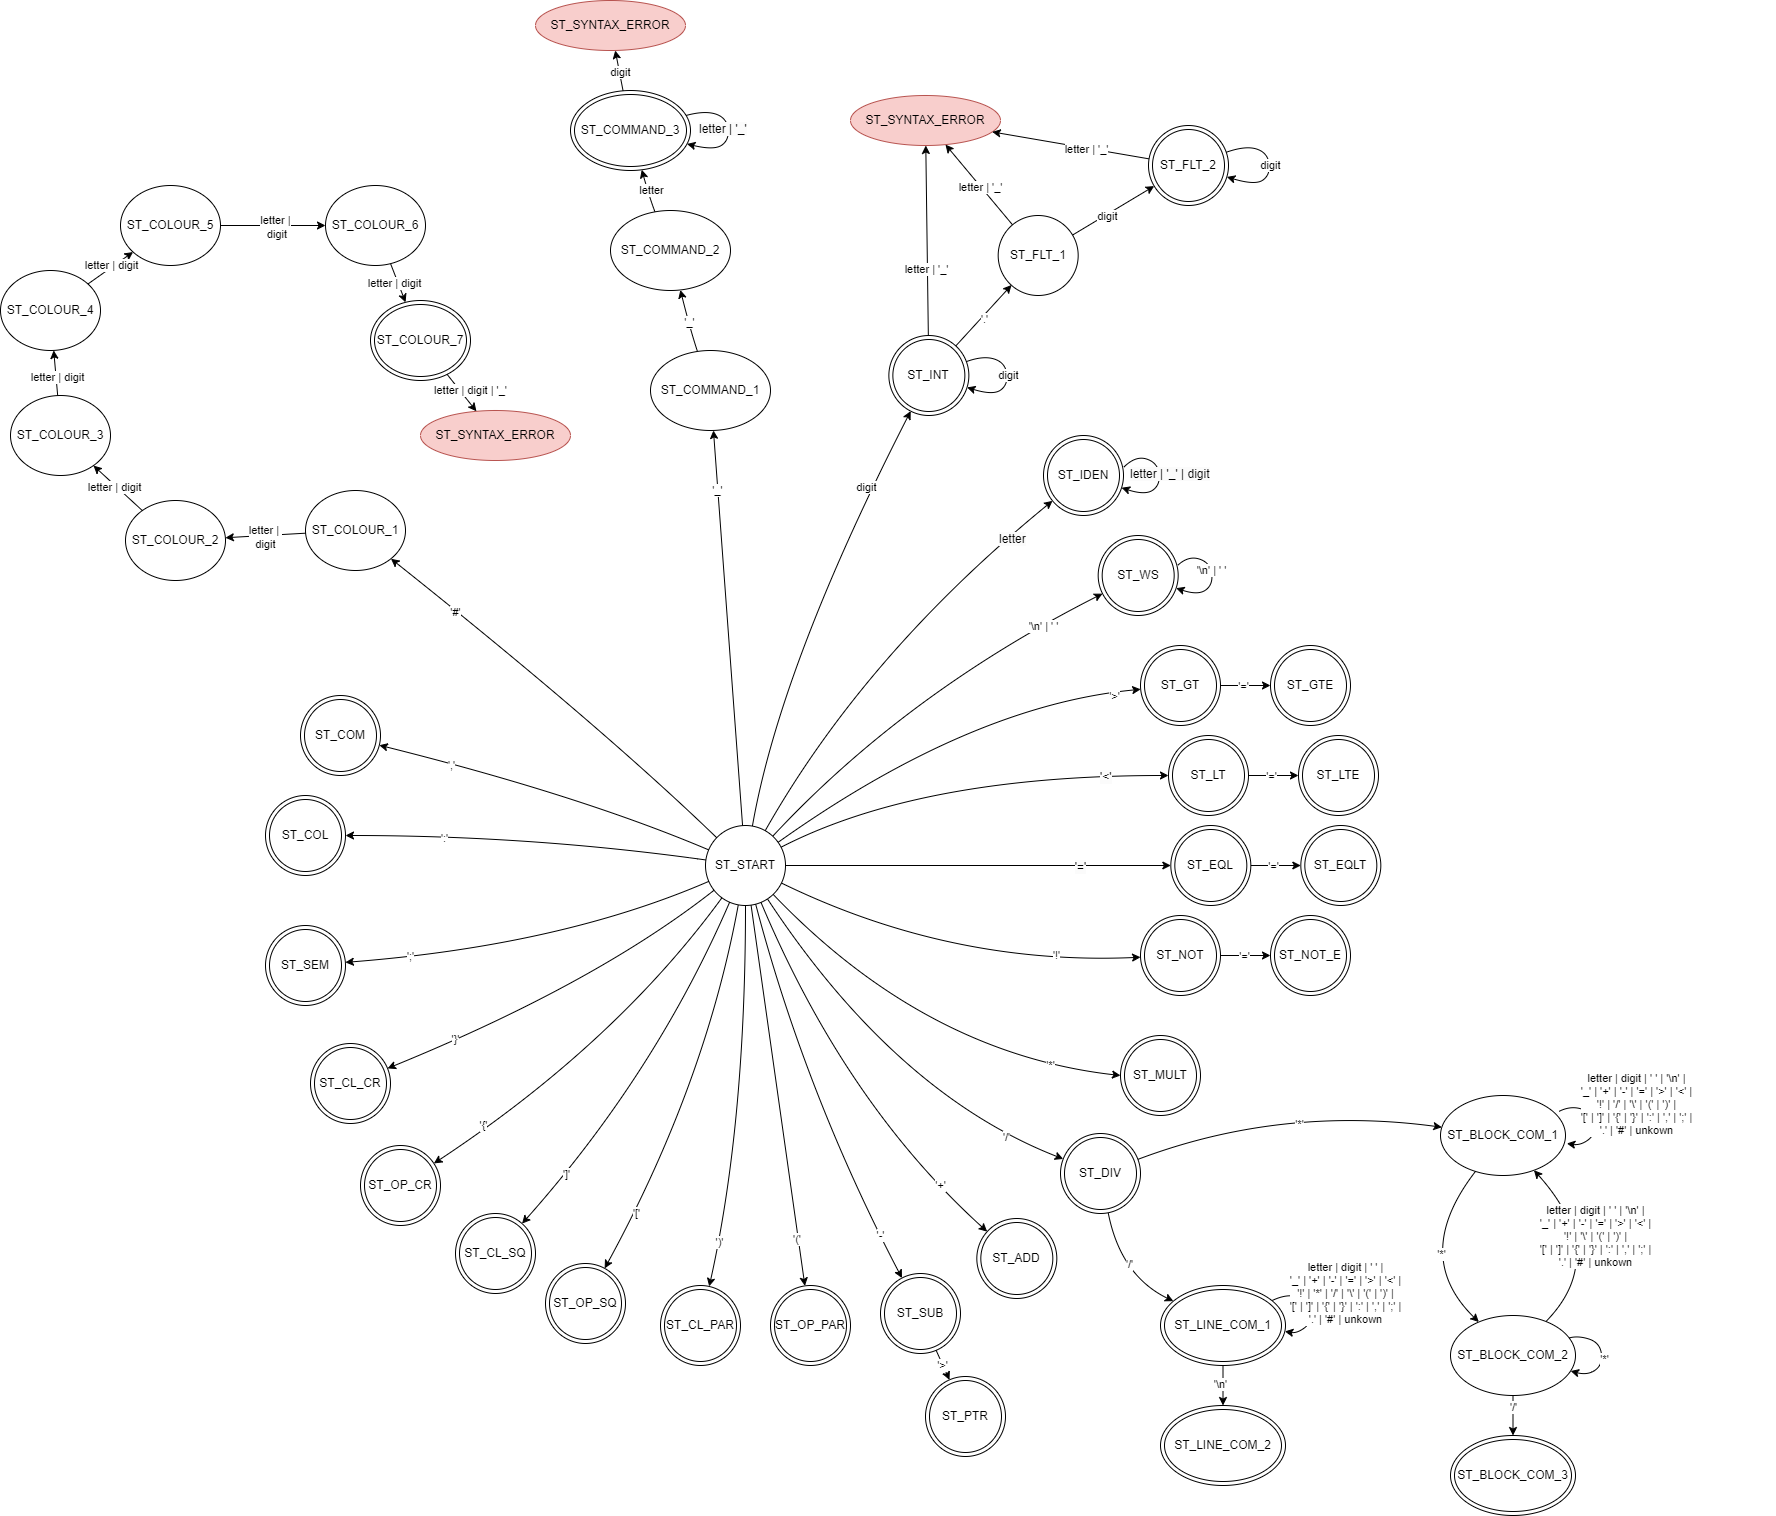
\includegraphics[width=15cm]{DFSA.png}
    \caption{DFSA}
    \label{DFSA}
\end{figure}

\section{Implementation}
During the implementation of the lexer, importance was given to adjustability and modification of the DFSA, more specifically the transition table. The idea was that new transitions or states could be added or changed without the need to change the transition table manually.

Firstly, the states shown in the DFSA are specified in the "Utility/types/States.h" file, as enums with st\_string allowing for enum-to-string conversion. The lexemes which direct the transitions can also be found in a similar file, "Utility/types/Lexemes.h".

The transition table is generated as a 2d array based on the number of enums specified for the states and lexemes, with lexemes specifying the number of columns, and states specifying the number of rows. All transitions are set to "Error" upon the creation/initialization of the table. The valid transitions are then specified in the Lexer's initTransitions() function, by using dfsa.addTransition() and specifying the row (current State), column (Lexeme), and next column (next state). This way transitions can be added or removed through this function, and the transition table is generated automatically.

\subsection{Lexical Process}
The basic premise of the lexer is that it stores previous states in a stack and new states are passed in per character read. Final states are similar to check points where if the lexer were to find an error state then the rollback until the last checkpoint is carried out.

The Lexer initially passes the "Syntax\_Error" state which is first placed to ensure the case that if no checkpoints are reached that would indicate that there was an un-tokenizable input. The first state will always be the "ST\_START", the lexer will then read a single character generating a lexeme for each one. Using the transition table with the current state and generated lexeme, the lexer can deduce the next state as if traversing the graph in the above figure [Figure \ref{DFSA}]. During this process, the last state is stored in the state stack. If that state is part of the designated final states (checkpoints) then the state stack is cleared before pushing the state. This is because the rollback is only interested until the last checkpoint so any states before that can be removed.

This process is repeated each time each character is added to a string buffer. This is done until a transition that is not listed is reached, in other words when the next state becomes the "ST\_Error" state. At this point, the Lexer rolls back to the last checkpoint removing a character from the buffer per removed state. If no checkpoint is reached then this is not a valid string and an error is raised. Else a token is mapped to the string using the state-token map. For certain tokens further validation is carried out; commands are further validated and given more specialised tokens if the command is valid, identifiers are checked to be either keywords or just identifiers (variable and function names), and colour literals are checked to hold valid hexadecimal characters.

It is important to note that if the transition table results in a "ST\_SYNTAX\_ERROR" the lexer raises an error since these indicate invalid strings. Another thing one may notice is that the generated tokens narrow down the strings as much as possible and do not group tokens, for example calling symbols such as ',', '.', ';' as punctuation since this helps the parser later on.

The process of combining characters into tokenised strings repeats until the lexer reaches the end of the inputted program string. The resulting list of tokenised strings is then returned.

The Lexer provides a way to debug this process by providing a display of the transition table and printing the process of using the transition table for each character. The function of showing each step can be enabled or disabled in the GenerateTokens function by setting the debug parameter to true/false. Both are on in the Lexer\_Tester executable.



% ==================================================================================
%                 Parser
% ==================================================================================
\chapter{Parsing}
The implemented parser is made up of mostly 2 parts, the abstract syntax tree and the parser itself. The parser also comes with the virtual parent implementation of the visitor class that future visitors will inherit, one of which is the display visitor which will be used to confirm that the parser is working correctly.

\section{Abstract Syntax Tree}
The AST Tree is based on the first Python code example. The tree is built out of hierarchical classes of all children belonging to the AST\_Node parent. Most child classes only serve to abstract and connect smaller subtrees. each level of the tree essentially serves as an abstracted container for the nodes below, for example, a statement may contain a while loop which in turn is made up of a condition expression and a block etc... 

It is the leaf nodes that contain proper values, these being nodes such as variables, integers and operand nodes. Certain higher-level nodes do store some values such as function declarations that hold types as well as identifiers. On this note, the reason that certain nodes seem to contain values that could be replaced with child nodes, such as how the function declaration node contains an identifier string instead of an identifier child node is due to the visitors. Although the identifier string may seem to serve the same purpose as the equivalent child node, the traversal/handling needs to be different, hence the easiest solution is to separate the two.

Certain nodes also hold a length variable. This is mostly used during the implementation and integration of arrays as it helps the flow of information and simplifies the visitors.

To allow choices when it comes to definitions such as how both write and write\_box are included as choices in the WriteStatement, the tree uses sub-hierarchies where the parent is virtual so the children can then be switched about without affecting the parent tree. This can be seen most clearly with the statement definition as AST\_Statement is itself a virtual class with its children being the different choices.

Another thing that might have been observed is that the AST tree implementation may differ slightly from the normal Visitor-ASTtree design pattern. This is because the tree itself is what handles the visitor's traversals, as it is the tree's accept functions that decide where the visitor should visit next instead of the traversal being handled more recursively by the visitor. Although this implementation may be slightly usual it did have its benefits as the visitors no longer needed to handle traversal as this was set once universally in the tree itself. This allowed for cleaner code and less repetitiveness although it did come at the cost of complexity as more thought was needed on the creation of the traversal structure since this needed to be compatible with all future visitor implementations.

One slight flaw that the nodes have is that it may be common to see multiple public statements when initialising the node classes, this was due to how the tree was structured before, where variables and the like were set as private. It was then later decided that these should be set to the public to easily access and change the values without needing the implementation of getters and setters. Hence the private keywords were replaced with public, although this doesn't affect the code's execution, it was worth mentioning.

\section{Parser}
Parsing is pretty straightforward in its implementation. Each Node has its own part in the parser. If these are fairly large they would usually warrant their own function. Otherwise, they would usually fall under one of the switch cases in the parent statement that contains the choices (such as parseStatement).

One key aspect is consistent across all nodes in the parser: if a parse function fails to find the correct first or second term, it resets the token list index and returns a nullptr. This approach is crucial for handling scenarios where the program needs to verify if the parsed item conforms to a specific type.

For instance, imagine the program needs to determine if the next tokenized set of strings forms a "Statement". It iterates through each potential statement choice to validate if the input aligns. If the initial tokenized string doesn't match any of the expected statement types, likely, the subsequent string isn't a statement either.

However, if the parser encounters a situation where it's parsing a construct and doesn't encounter the anticipated subconstruct (e.g., a variable declaration not followed by an expression), it raises an error. In this context, it's more probable that the user inputted an invalid structure, warranting an error message.

An extension which was added to the parser was the inclusion of the length variable in the AST\_Tree. This was added later to be used in the semantic and code generation visitors, to handle arrays. As a general note when the length is set to -1, this would indicate a normal expression or variable call meaning that the variable is not of type array. If the size is 0 or above, the visitors are dealing with arrays.

\subsection{Verification Functions}
The parser in general is rather hard to give a general explanation which could be used throughout it, since many of the different functions are unique, having to deal with the different rules. Although there is one set of functions that is frequently used throughout the parse functions. These are the verification functions, which include the verifyType(), verifyNext() and verifyNode(). These functions serve to make the code more readable as they condense the verification of different constructs and the error messaging in a single function.

\begin{itemize}
    \item \textbf{verifyType()}: This function checks that the next token is a type-related token such as a bool.
    \item \textbf{verifyNext()}: This function takes a given token type and makes sure the next token is related the same as that token. This is the most commonly used one. Like the other verify functions it also returns the token if it is valid, but this is not always used as many tokens do not need to be stored in the tree such as the ':' in a declaration statement.
    \item \textbf{verifyNode()}: This is the last verify function, used to deal with the event that a parse function was unable to parse the expected item. Since the Parser follows a rollback system and does not always immediately resort to an error statement, this function checks whether parsing has been successful.
\end{itemize}

Each function takes 2 sets of different parameters which change on what the error message should display. These include elements such as the location of the calling function, a secondary location to show more specifically where, and the message itself.

\section{Deviations}
There are a couple of deviations made from the original EBNF. These were made either to make certain parts clearer, and easier or to fix what are presumed to be some small mistakes.

The first is that the unary expression was changed to no longer be on an expression but on a factor since how it was stated would not make sense as there are no brackets around the expression to contain what the unary operator is affecting. Changing it to make use of a factor solves this as one of the choices is a subexpression which is the exact solution.

Another change is that function declarations are no longer followed by a block but a sudo-equivalent called a weak block. The virtually performs in the same manner but it allows the semantic visitors later on to decipher the two since the first block in a function declaration has different requirements compared to other blocks.

The last change was made to 〈PadWidth〉,〈PadHeight〉and,〈PadRead〉as these were removed from the choice in factor since they were already defined in 〈Literal〉.

\section{Visitor}
Together with the AST\_Tree, the virtual visitor is also defined. This will be the parent for all visitors defined later on. It is important to know that certain nodes in the AST\_Tree contain multiple visit statements. These are for visitors such as the code generator later on. They act as checkpoints throughout larger constructs, these are used to store values such as current instruction numbers for loops and the like so that statements such as jumps can be included. It is for this reason that the visitor has multiple visits for certain nodes. Each visit acts as a checkpoint for the visitor to take an action. A simple example would be at the start and end of a block, where a visitor needs to create and then destroy a scope.

\section{Display Visitor}
The Display Visitor is the most basic visitor implementation and is included with the Parser implementation. Through the Display Visitor, one can obtain a visual representation of the AST\_Tree. Effort was made to attempt to display the tree structure in a readable format with the branches and nodes being indented with symbols to define the levels better. That being said the order of traversal shown in the output may be slightly unintuitive meaning that the output of operations is in a different order than what would be expected and can be slightly hard to read. This is because the traversal was created to be optimized to work more effectively for the segment and code-generation visitors. That being said this does have the added benefit of visually seeing how the later visitors will traverse the tree as well as giving an abstract look at how the code will be generated.

% ==================================================================================
%           Semantic Analysis
% ==================================================================================
\chapter{Semantic Analysis}
The semantic analysis is done through a visitor similar to the Display Visitor from before. The implementation is contained inside the Semantic folder. Semantic\_Scope\_Functions.cpp holds some utility functions that are used while the main implementation is stored in the relative cpp file.

\section{Scopes}
In order to properly decipher between the scope levels, the visitor makes use of a stack. More specifically 2 stacks but only 1 is ever in use at a time. The function scope stack is to prevent function declarations from accessing variables from the main scope. The function scope stack is only activated when a function declaration is currently being processed. This isolates the two stacks and also helps in checking commands such as the return statement, as this should only be called when we are currently in a function scope.

Each scope holds an array of variable\_t structs which hold variable values that are important for semantic analysis, such as the name and type, length is also used to specify if the variable is an array. Each scope holds a counter of the number of variables, this is mostly used during code generation to allocate variables at the end start of a scope.

\section{Global Functions}
Since functions can only be created in the main scope, at least in my implementation, functions are not stored in scopes but in a separate array which can be accessed from anywhere. Similarly to scopes, the global functions array holds a list of function\_t structs each holding information that is used for either code generation or semantic analysis. Functions hold their names, and a list of parameter types and for each a length to decipher from arrays. The return type similarly has both a type and a length for the same reasons.

\section{Type Stack}
Since traversal is already taken care of through the AST\_Tree all there needs to be done now is push and pop types during traversal to a global stack as needed. For example, take the following case:

$$x = 2+1$$

The AST\_Tree is already set to traverse the statement in this order: 

$$1, 2, +, x$$

so all we need to do is push the types of the "simple" nodes to the stack and then pop when we want to compare. So the stack would go through the following
\begin{itemize}
    \item push int
    \item push int
    \item pop, pop -> validate -> push result type
    \item pop expression result -> search for variable type -> validate
\end{itemize}


This is only a simple example, but it can be seen how this process can be extended for more complicated cases.

\section{Important Symentaic Notes}
Certain restrictions made during semantic analysis are not listed in the requirements and were done through creative freedom in the implementation.

Firstly variables and elements of type float are compatible with variables of type integer. This means that a variable of type float can be assigned an integer number. Integers and Floating points can also be compared and multiplied as well as all the other operations. That being said if a floating point and an integer are multiplied/divided/added/subtracted, the result is a floating point number. Division always returns a floating point number as well since most commonly division results in a non-whole number/result.

Another thing is that arrays also cannot be compared or used with any operations unless an index is specified. This was as comparing entire arrays with single values or adding with single values did not make sense, hence this was not allowed. Another thing related to arrays is that they cannot be directly printed, this will be further discussed in the code generation part. The semantic analysis also takes into account array lengths, when either pushing or assigning whole arrays. This is to make sure that if a function takes a certain array length and type then only a matching array can be passed. 

An important note is return types, although the effort could have been made to check for return statements in if-statements and other cases, this was deduced to take too much time and not worth the effort for minimal effect. How returns are currently handled is that if a function has a return type in its main scope then the function is valid as it has at least one return. The main scope is found through the tab counter as the main scope is always at the same tab number. To properly implement return types, a proper visitor would probably be needed whose job is simply to check that a function declaration has a proper return type.


% =================================================================================
%            Code Generation
% ==================================================================================
\chapter{Code Generation}
The purpose of the code generation is to create a vector/list of strings each holding a command. This list of commands is generated from the AST\_Tree where each node has its own dedicated instruction or set of instructions.

\section{Carried Over}
The Code Generator works largely in a similar manner to the semantic analyser. In fact, the main\_scope and function\_scope stacks are carried over from the semantic visitor, this time used to calculate the scope and variable indexes of called variables. The global functions are also carried over, this time used to specify the number of parameters passed during a function call. This is because it is easier to calculate the number of variables, especially when arrays are involved, from the global function call rather than trying to count the number of expressions in a function call.

\section{Patching Method}
The best way to create instruction that depends on future information is to not create them at all, well at least at first. The patching method operates by inserting a placeholder instruction where additional information is required, such as when a scope needs the number of variables declared to allocate them. The instruction number for this blank instruction is then stored inside the instruction stack. It is at this point where the true uses of the multiple checkpoints/subvisits that certain nodes hold come into use. These blank instructions are then filled by another visit later on where by poping the instruction stack it is able to update that instruction with the necessary data. One example of this is the if statement where the jump condition after the if's expression needs to be updated with the number of instructions to skip in the if block. At first, a blank instruction is stored but this is then filled by the visit at the end of the if which calculates the instruction difference and sets that as the push.


\section{Scopes}
Scopes usually follow a similar format each time and use the patching method. Scopes inside the virtual machine are specified through frames, where upon opening a frame the variables declared need to have their memory pre-ellocated before the statements start. To do this the scope inserts a blank function at the start before the "oframe" instruction which is then filled by the close scope visit. Function declarations have a similar format but use alloc instead of the normal frame since a function call already opens a frame.

\section{Minor Imperfections}

There are a couple of limitations which the compiler doesn't account for. The first one is that although there exists a print array function, there is no easy implementation for it with how the visitors are set up. Semantically it wouldn't be a problem as the type stack stores the expression length, hence it would know that the expression includes an array, but this was not included in the code generator. This means that the print node would not be able to tell whether it is dealing with an array or a normal 1-value expression hence it wouldn't be able to include the proper print. It is for this reason that the printa statement was not used. Other commands weren't put to use such as the increment, modulus and decrement, as well as others. Since these weren't listed in the EBNF then it was deemed unnecessary to include them.

\chapter{Worked Example}
Below can be seen an example code snippet that will be parsed, semantically checked and compiled as an example of how the created compiler will process a given code snippet.

\begin{minted}[frame=lines,framesep=2mm,baselinestretch=1.2,bgcolor=LightGray,
fontsize=\footnotesize,linenos,breaklines=true]{c++}
fun inc_array (x : int[8]) -> bool{
    for(let i:int = 0; i < 8; i = i+1){
        x[i] = i;
        __print x[i];
    }
    return true;
}

let list_of_integers : int[8] = [0];
let result:bool = inc_array(list_of_integers);
\end{minted}
In the following explanations not every part of the item will be described in great detail as this would be too long. Hence only certain elements considered to be important will mostly be explained. Of course, this code can be run through the compiler to visualise the output better.

\section{Lexical Analysis}
To better visualise the lexical analysis process one can enable or disable the debugging mode through the boolean parameter in GenerateTokens(). Another thing to keep in mind is that the transition table can also be displayed through displayTable(), but this is too large to be shown here.

\begin{minted}[frame=lines,framesep=2mm,baselinestretch=1.2,bgcolor=LightGray,
fontsize=\footnotesize,linenos,breaklines=true]{c++}
0   [f]   letter            START             ST_IDEN           
1   [u]   letter            ST_IDEN           ST_IDEN           
2   [n]   letter            ST_IDEN           ST_IDEN           
3   [ ]   space             ST_IDEN           ERROR             

3   [ ]   space             START             ST_WS             
4   [i]   letter            ST_WS             ERROR             

4   [i]   letter            START             ST_IDEN           
5   [n]   letter            ST_IDEN           ST_IDEN           
6   [c]   letter            ST_IDEN           ST_IDEN           
7   [_]   underscore        ST_IDEN           ST_IDEN           
8   [a]   letter            ST_IDEN           ST_IDEN           
9   [r]   letter            ST_IDEN           ST_IDEN           
10  [r]   letter            ST_IDEN           ST_IDEN           
11  [a]   letter            ST_IDEN           ST_IDEN           
12  [y]   letter            ST_IDEN           ST_IDEN           
13  [ ]   space             ST_IDEN           ERROR  
\end{minted}

Here is an example from the given code on how the lexical process is done. Each column holds the required data for that transition. The first row contains the letter index currently being traversed, the second column holds the letter in question. The last 3 columns hold the generated lexeme, the current state and finally the next state as dictated by the transition table.

Each new iteration (indicated by the blank space) starts with the Start state as the default current state. If we take an example with the fun keyword, it can be seen how the Lexer processes each letter generating the next state. This is done until the Error state is encountered which rolls back to the last acceptable final state, this being ST\_IDEN.
\begin{minted}[frame=lines,framesep=2mm,baselinestretch=1.2,bgcolor=LightGray,
fontsize=\footnotesize,linenos,breaklines=true]{c++}
============================ TOKEN LIST ============================

0     FUN                [fun]
1     WHITESPACE         [ ]
2     IDENTIFIER         [inc_array]\sec
\end{minted}
These are the generated tokens for the before-listed example. As it can be seen fun was not left as an identifier but changed to be linked to a more specific token called FUN which denotes the function keyword. As inc\_array does not specify any keyword it was left to be an identifier.

\section{Parsing}n
To create the AST\_Tree, the parser makes use of the generated token list and creates nodes connecting. Both the code and the AST Tree are too long to include here in full hence it is recommended to have them side by side while going through the explanation

Let's take an example of the function declaration. Hence the following explanation will be related to the code snippet at "Parser/Parse\_Statement" in the parseStatement function, function case (around line 480).

The case will start off with consuming the token used during the switch case's condition. This would be FUN keyword. It then proceeds to check that the identifier is in the correct position using the verifyNext which checks that the next token in the list matches the token type passed as a parameter. An open parenthesis '(' then follows the identifier. There are two cases that may follow, in the case the function takes no parameters then the close parenthesis ')' should be the next token, else the function parses the formal parameters.

Formal Parameters are parsed in this manner, the function checks for an identifier, a colon and a type in that order. These are used to create the formal\_param\_node. The function then checks for arrays through the square bracket, ensuring they follow the EBNF as before. After each successful formal parameter parsing the function adds that node to the formal\_params\_node and repeats the process if a comma follows it, else it ends the loop by adding the formal\_params\_node to the function declaration.

The function then checks for a return type by looking for a pointer followed by a type, the type of course could be an array which is in turn processed the same way as array parameters. The rest of the parsing is then left to the parseWeakBlock which parses a weak block node and returns it. The node is verified and finally attached to the function declaration node. this newly created function declaration node is then returned to whatever was the calling function.

Other parsing elements are done in a similar fashion where the conditions and format are hard coded into the compiler.

\section{Semantic Analysis}
In this section, there is not a lot of visual feedback as compared to the previous parts. Hence the explanation will be a bit more vague in certain aspects. For this section, we will be discussing the function call and how it would be semantically parsed.

For the function call the assumption in place is that the function declaration has already been traversed and semantically checks, with its signature put into the global function stack. In the AST\_Tree generated at the function call it can be seen that the parameters of that function call will be traversed before the function call itself. This means that the types of the parameters should have been pushed to the type stack from right to left so that the first parameter's type is at the top of the stack. All the visitor needs to do therefore is to first find the function signature from the global function array and make sure the identifier exists. 

Once the signature is found there are several steps to be done, first, the child node list containing the function call parameters should be compared to the signatures parameter list to make sure the correct amount of parameters are being called. Secondly, the visitor can now pop the types from the type stack, for each comparing the length and type to that of the signature's parameter. Once this is successful the visitor just needs to push the signature's return type to the type stack. This is because the expression in which the function call is contained will need the type for comparisons, assignments and the like.

\section{Code Generation}
For code generation, the visitor follows a similar design to that of the semantic analysis, although this time repurposed for code generation. The same scope stacks and global function list used in the previous visitor are once again used. Tree traversal also doesn't need to be taken into account as once again it's taken care of from the tree itself. 

The for loop is one of the best places to see how the code generation works as it has multiple visit functions throughout it.

\begin{minted}[frame=lines,framesep=2mm,baselinestretch=1.2,bgcolor=LightGray,
fontsize=\footnotesize,linenos,breaklines=true]{c++}
// ----------------------------------------------------------------------------------------- Start For
void Gen_Visitor::visit_start_for (const AST_For* node){
    getCurrentScopeStack().push_back(scope_t{});
    addBlankInstructions(); // number of variables for oframe
    pushInstructionNum(getCurrentInstructionNumber());

    addNewInstruction("oframe");
}
\end{minted}
The start of the for loop is where the for loop scope is created and is called before any of the other components are called. The blank instruction is inserted into the instruction array to be later updated with the number of variables that the oframe should allocate.

\begin{minted}[frame=lines,framesep=2mm,baselinestretch=1.2,bgcolor=LightGray,
fontsize=\footnotesize,linenos,breaklines=true]{c++}
// ----------------------------------------------------------------------------------------- Jump For
void Gen_Visitor::visit_jump_for (const AST_For* node){
    pushInstructionNum(getCurrentInstructionNumber());
}
\end{minted}

The jum\_for is called before the expression node but after the declaration. This is to save the instruction number of where the end of the loop should jump to to continue looping.
\begin{minted}[frame=lines,framesep=2mm,baselinestretch=1.2,bgcolor=LightGray,
fontsize=\footnotesize,linenos,breaklines=true]{c++}
// ----------------------------------------------------------------------------------------- Skip For
void Gen_Visitor::visit_skip_for (const AST_For* node){
    addNewInstruction("push #PC+4");
    addNewInstruction("cjmp");

    addBlankInstructions(); // instruction to jump to to skip loop
    pushInstructionNum(getCurrentInstructionNumber());
    addNewInstruction("jmp");
}
\end{minted}
This visit statement takes care of the conditional jump. most conditional jumps follow this format, if the previous statement is true, the cjmp will skip the next jump instruction and allow the looping to continue. If the next jump instruction is not skipped then it is set to send the current command reader to the end of the for loop hence ending the loop. The large jump is of course set to a blank instruction as for now the program does not as of yet know the number of instructions which make out the for loop's block.
\begin{minted}[frame=lines,framesep=2mm,baselinestretch=1.2,bgcolor=LightGray,
fontsize=\footnotesize,linenos,breaklines=true]{c++}
// ----------------------------------------------------------------------------------------- End For
void Gen_Visitor::visit_end_for (const AST_For* node){
    int skip_instr = popInstructionNum();
    int jump_instr = popInstructionNum();
    int ofrm_instr = popInstructionNum();

    PatchNewInstruction(ofrm_instr, "push " + std::to_string(getCurrentScopeStack()[getCurrentScopeStack().size()-1].num_var));

    addNewInstruction("push #PC"+std::to_string(jump_instr - getCurrentInstructionNumber()));
    addNewInstruction("jmp");

    PatchNewInstruction(skip_instr, "push #PC+" + std::to_string(getCurrentInstructionNumber()+1 - skip_instr));

    addNewInstruction("cframe");
    getCurrentScopeStack().pop_back();
}
\end{minted}
The final visit is there to patch all the previously created blank instructions. As can be seen from the pop function the instruction numbers were pushed inside a stack so they need to be popped in the reverse order. The oframe instruction number is popped last and at that location number of variables inside the top-most scope in the scope stack are pushed so that the virtual machine can allocate. This also works for arrays as the num\_var variable is updated according to the length of an array as well.

The second instruction popped is the jump instruction and here the loopback address is calculated and added followed by a push. If the loop started at instruction number 7 and we are currently at instruction 20 then this would push the address PC-13 which would be where the loop needs to start again for a new iteration. This must be done before the skip is updated as the skip should skip to after the loopback jump. The skip is then another patch where the current instruction number is pushed replacing the blank instruction left at the start. 

The last thing the visitor will do now is to close the frame and remove the scope from the stack
\end{document}
